\documentclass[conference]{IEEEtran}
\IEEEoverridecommandlockouts
% The preceding line is only needed to identify funding in the first footnote.

\usepackage{cite}
% IEEEtran switches the body font to Times (ptm) via \rmdefault, but the
% classic PSNFSS Times metrics have no small-caps face, so the \scshape
% used by \section silently fell back to plain text ("I. Introduction"
% instead of true small caps "I. INTRODUCTION"). newtxtext is a modern
% Times-alike replacement that actually ships a small-caps design.
\usepackage{newtxtext}
\usepackage{amsmath,amssymb,amsfonts}
\usepackage{algorithmic}
\usepackage{graphicx}
\usepackage{textcomp}
\usepackage{xcolor}
\usepackage{booktabs}
\usepackage{multirow}
\usepackage{url}

\def\BibTeX{{\rm B\kern-.05em{\sc i\kern-.025em b}\kern-.08em
    T\kern-.1667em\lower.7ex\hbox{E}\kern-.125emX}}

% Forces a row break in the \author block (like \and, but starts a new,
% independently centered row) so a 5-author list lays out as 2 / 2 / 1
% instead of letting IEEEtran's automatic wrapping strand the last name.
\makeatletter
\newcommand{\linebreakand}{%
  \end{@IEEEauthorhalign}
  \hfill\mbox{}\par
  \mbox{}\hfill\begin{@IEEEauthorhalign}
}
\makeatother

\begin{document}

\title{BioMarkHER2: A Pathologist-in-the-Loop System for Quantitative\\
HER2 IHC Pre-Scoring Under Weak Supervision and CPU-Only Compute
\thanks{Funding acknowledgment withheld pending submission.}
}

\author{
\IEEEauthorblockN{J. S. Varughese}
\IEEEauthorblockA{
\textit{Department of Computer Science and Engineering} \\
\textit{Mar Baselios College of Engineering and Technology} \\
Thiruvananthapuram, India \\
johansvarughese.b23cs2135@mbcet.ac.in}
\and
\IEEEauthorblockN{Nadeema Jahan}
\IEEEauthorblockA{
\textit{Department of Computer Science and Engineering} \\
\textit{Mar Baselios College of Engineering and Technology} \\
Thiruvananthapuram, India \\
nadeemajahan.b23cs2146@mbcet.ac.in}
\linebreakand
\IEEEauthorblockN{Aiswarya M S}
\IEEEauthorblockA{
\textit{Department of Computer Science and Engineering} \\
\textit{Mar Baselios College of Engineering and Technology} \\
Thiruvananthapuram, India \\
aiswaryams.b23cs2111@mbcet.ac.in}
\and
\IEEEauthorblockN{Rishika Pratap Jadgale}
\IEEEauthorblockA{
\textit{Department of Computer Science and Engineering} \\
\textit{Mar Baselios College of Engineering and Technology} \\
Thiruvananthapuram, India \\
rishikapratapjagdale.b23cs2155@mbcet.ac.in}
\linebreakand
\IEEEauthorblockN{Dr. Jesna Mohan}
\IEEEauthorblockA{
\textit{Associate Professor, Department of Computer Science and Engineering} \\
\textit{Mar Baselios College of Engineering and Technology} \\
Thiruvananthapuram, India \\
jesna.mohan@mbcet.ac.in}
}

\maketitle

\begin{abstract}
Manual HER2 immunohistochemistry (IHC) scoring is subjective at its class
boundaries, and the equivocal 2+ category triggers a second, costly
confirmatory test. We present BioMarkHER2, an end-to-end AI-assisted
\emph{measurement} system for HER2 IHC intensity, built under two hard
constraints: no real whole-slide-image data yet exists for the clinical
site this project targets (84 slides, not digitized), and the development
machine is CPU-only. The system comprises classical stain-based
preprocessing, a weakly-supervised segmentation model trained without any
pixel-level annotation, an evaluation framework combining conformal
prediction, cross-group stain-variation analysis and offline ASCO/CAP
mapping, and a local review-viewer web application through which a
pathologist inspects the model's output beside a classical control and
records a confirmed score. The system's central design principle --
assistive, never autonomous -- is formalized as a strict functional
boundary between measurement and diagnosis and enforced as executable
tests, not only as documentation: no API response or UI anywhere is
permitted to carry a field named \texttt{score}, \texttt{her2\_score},
\texttt{verdict} or \texttt{diagnosis}, checked on every test run. We
report results across the full pipeline, an honest coverage accounting
against the project's original nine-item brief, a validity-threat analysis
organized by the standard construct/internal/external/statistical
taxonomy, and the items that remain genuinely blocked on data no
engineering effort can substitute for, rather than on missing code.
\end{abstract}

\begin{IEEEkeywords}
digital pathology, HER2, immunohistochemistry, weak supervision, conformal
prediction, human-in-the-loop, clinical decision support
\end{IEEEkeywords}

\section{Introduction}

HER2 status determines eligibility for HER2-targeted breast cancer therapy
and is assigned by pathologists from immunohistochemistry (IHC) membrane
staining on a 0/1+/2+/3+ scale, per the ASCO/CAP guideline
\cite{wolff2018}. The 2+ ("equivocal") category cannot be resolved from
IHC alone and triggers a second, more expensive confirmatory test
(FISH/ISH); manual scoring at the 0-versus-1+ and 2+-versus-3+ boundaries
is known to vary between observers. Against the backdrop of a broader,
well-documented shift toward AI-assisted diagnosis in digital pathology
\cite{bera2019}, this motivates a quantitative, AI-assisted pre-scoring
tool -- one that measures staining and hands the measurement to a
pathologist, rather than one that scores autonomously.

This paper reports on BioMarkHER2, a final-year academic system built with
a specific medical college as its clinical reference point, under two
constraints that shape nearly every engineering decision in the system:

\begin{itemize}
\item \textbf{No real whole-slide-image data exists yet.} The reference
  site's 84 slides are not digitized. Every result in this paper is built
  and validated against an approved public stand-in dataset,
  HER2\_IHC\_40X, until real slides arrive.
\item \textbf{The development machine is CPU-only.} No GPU is available.
  Every model, batch size and epoch count in this system is sized to
  actually complete on a laptop CPU.
\end{itemize}

Rather than treat these as footnotes, we treat them as first-class design
constraints and report their consequences explicitly throughout: which
components are software-complete but only run at smoke scale, which
objectives are fully exercised, and which are genuinely blocked on data
rather than on missing engineering.

The system's overriding design principle is stated once and then enforced
everywhere:

\begin{quote}
\emph{This is a pre-scoring assistive tool that a pathologist reviews and
confirms -- never an autonomous final-scorer.}
\end{quote}

Concretely, this is not a policy documented in prose. No code path anywhere
in the system is permitted to produce a field named \texttt{score},
\texttt{her2\_score}, \texttt{verdict}, or \texttt{diagnosis}; a test suite
scans the live application's JSON output on every run and fails the build
if one ever appears. A pathologist review can only be recorded through an
explicit, human-initiated submit action. We describe this enforcement
mechanism in Section~\ref{sec:app} because we consider it as much a
contribution as any individual model result: a framing constraint that is
only ever documented, not tested, is a framing constraint a well-intentioned
future edit can erode without anyone noticing.

This paper makes four contributions: (i) a complete, reproducible pipeline
from raw IHC patch to a pathologist-facing measurement, built entirely
under weak supervision and CPU-only compute; (ii) a head-to-head
architecture comparison that resolves a diagnosed resolution failure on
HER2 IHC's most clinically consequential class; (iii) an evaluation
framework -- conformal prediction, stain-variation analysis, offline
clinical-guideline mapping -- that reports calibrated uncertainty and
expert agreement rather than a bare accuracy number; and (iv) a systematic
validity-threat analysis and honest coverage accounting against the
project's original brief, so that what remains blocked on data, rather
than on engineering, is stated explicitly rather than left implicit.

\section{Related Work}
\label{sec:related}

\textbf{Computational pathology and HER2 IHC scoring automation.} AI-assisted
digital pathology has matured rapidly as a diagnostic and precision-oncology
tool \cite{bera2019}. Automated HER2 scoring work within it typically
targets patch- or slide-level classification of the 0/1+/2+/3+ label
directly, including pyramid-sampling convolutional architectures for
whole-slide HER2 scoring \cite{selcuk2024} and multi-stage CNN classifiers
for HER2 category prediction \cite{mridha2022}. Pixel-level segmentation of
the staining pattern itself is comparatively unexplored, in part because
pixel-level HER2 IHC annotations are not publicly available at scale --
the gap this system's weak-supervision pipeline (Section~\ref{sec:phase2})
is built to work around, following a broader precedent for deriving dense
segmentation targets from patch-level classification labels in
histopathology \cite{han2021}.

\textbf{Human-in-the-loop clinical decision support.} Systems in this space
generally separate a measurement or triage step from the diagnostic
decision itself; our review-viewer follows the same separation, with the
"no score field" rule as its literal, tested boundary
(Section~\ref{sec:app}), rather than a convention left to interface design
alone.

\textbf{Stain variation.} Colour and intensity variation across scanners
and staining protocols is a well-known confound in computational pathology;
recent generative approaches address it directly, e.g., with
cycle-consistent adversarial networks for multi-domain stain normalization
\cite{hetz2024}. We take a complementary, non-generative approach --
estimating a per-patch stain descriptor \cite{macenko2009} and using it
both to characterize cross-group variation (Section~\ref{sec:phase4}) and
to reweight conformal calibration evidence (Section~\ref{sec:conformal})
-- rather than learning a normalizing transform.

\textbf{Conformal prediction for medical imaging.} Conformal prediction
\cite{vovk2005} provides distribution-free, finite-sample-valid
uncertainty for exactly this kind of assistive setting; recent work wraps
segmentation output with morphological prediction sets
\cite{mossina2025} or quantifies region-level uncertainty for U-Net-based
clinical tools \cite{borden2026}, both as general-purpose, task-agnostic
layers over an already-trained model. We build instead on a
task-specific application of conformal prediction to binary, image-level
HER2 status classification \cite{pintawong2025}, generalizing it to
pixel-level, five-class segmentation output (Section~\ref{sec:conformal}).

\section{System Overview}

\begin{figure}[t]
\centering
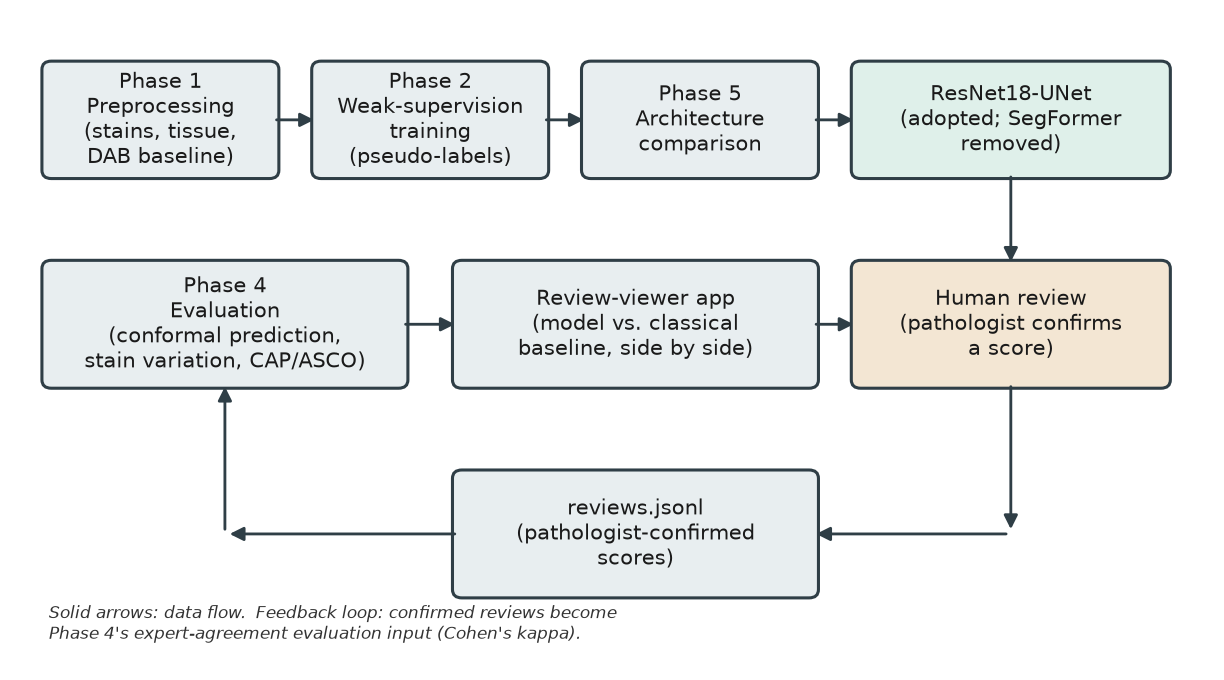
\includegraphics[width=\columnwidth]{../figures/pipeline_diagram.png}
\caption{System pipeline. Phase 1 preprocessing feeds Phase 2's
weak-supervision training; two architectures were compared head-to-head
(Phase 5) and ResNet18-UNet was adopted. Phase 4 evaluates the model;
the review-viewer application is the pathologist-facing surface, and
confirmed reviews feed back into Phase 4's expert-agreement evaluation.}
\label{fig:pipeline}
\end{figure}

Fig.~\ref{fig:pipeline} shows the system end to end. Phase 1
(Section~\ref{sec:phase1}) turns a raw RGB IHC patch into a tissue mask, a
classical DAB-threshold intensity classification, and area percentages.
Phase 2 (Section~\ref{sec:phase2}) trains a segmentation model on
pseudo-labels derived from Phase 1, since no pixel-level annotations exist.
Phase 5 (Section~\ref{sec:phase5}) compares two candidate architectures
head-to-head and selects one. Phase 4 (Section~\ref{sec:phase4}) evaluates
the selected model with conformal prediction, stain-variation analysis, and
offline ASCO/CAP mapping. The review-viewer application
(Section~\ref{sec:app}) is the pathologist-facing surface that ties these
together and is the only place a HER2 score is ever recorded, by a person,
on explicit submission.

\subsection{The Design Principle, Stated Formally}
\label{sec:principle}

We state the system's one enforced rule as a functional boundary, since a
precise statement is what makes it testable rather than aspirational. Let
$g_\theta: x \mapsto \hat p$ denote the entire measurement pipeline --
preprocessing, the segmentation model, and evaluation -- mapping an input
image $x$ to a vector of per-class area percentages and calibrated
prediction sets $\hat p$. Let $h: (\hat p, \text{clinical judgment})
\mapsto \text{score} \in \{0,1{+},2{+},3{+}\}$ denote the pathologist's own
act of scoring. \textbf{The system's one invariant is that no
composition of functions reachable from a live API request implements any
approximation of $h$}: $g_\theta$ is never followed, inside the system, by
a step that collapses $\hat p$ to a categorical score. Section~\ref{sec:app}
describes how this is checked, not merely declared, on every code change.

\section{Phase 1: Data and Preprocessing}
\label{sec:phase1}

\subsection{Dataset}

We use HER2\_IHC\_40X, $\approx$11{,}000 (10{,}997) 1024$\times$1024 RGB IHC
patches at 40$\times$ magnification, organised into four intensity folders
with a slide-score filename prefix, as an approved substitute while the
reference site's slides remain undigitized. The dataset provides no
pixel-level masks and no slide identifiers -- both facts propagate into
every later phase's evaluation methodology and are restated where they
matter, rather than only here. Fig.~\ref{fig:datasetdist} shows the class
distribution of the 2{,}200-patch test split used throughout this paper.

\begin{figure}[t]
\centering
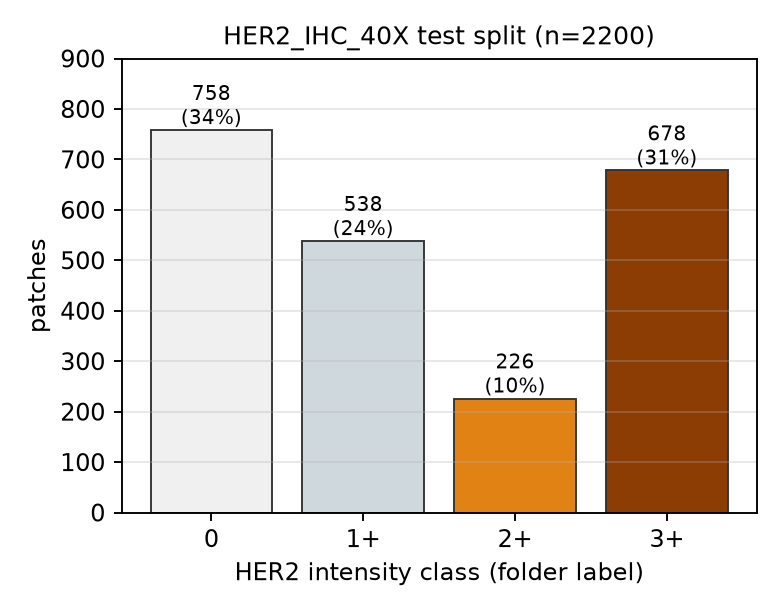
\includegraphics[width=0.75\columnwidth]{../figures/dataset_distribution.png}
\caption{HER2\_IHC\_40X test-split class distribution (folder label).
Moderate (2+) -- the class that decides reflex FISH testing -- is the
rarest, at 10\% of patches.}
\label{fig:datasetdist}
\end{figure}

\subsection{Stain Deconvolution}

HER2 IHC is dual-stained: haematoxylin (nuclear counterstain, blue) and DAB
(the HER2 signal, brown). We separate the two by Ruifrok and Johnston
colour deconvolution \cite{ruifrok2001} in optical-density space.
Fig.~\ref{fig:deconv} shows this decomposition on a real, strongly-stained
patch: the recovered DAB channel is the quantity every intensity class and
every area percentage in this system is a function of. Stain normalization
(Macenko \cite{macenko2009}, Reinhard \cite{reinhard2001}) is implemented
but defaults to off, since HER2\_IHC\_40X is single-source and
normalization would shift the exact optical densities the intensity
thresholds are defined on without correcting any real variation.

\begin{figure}[t]
\centering
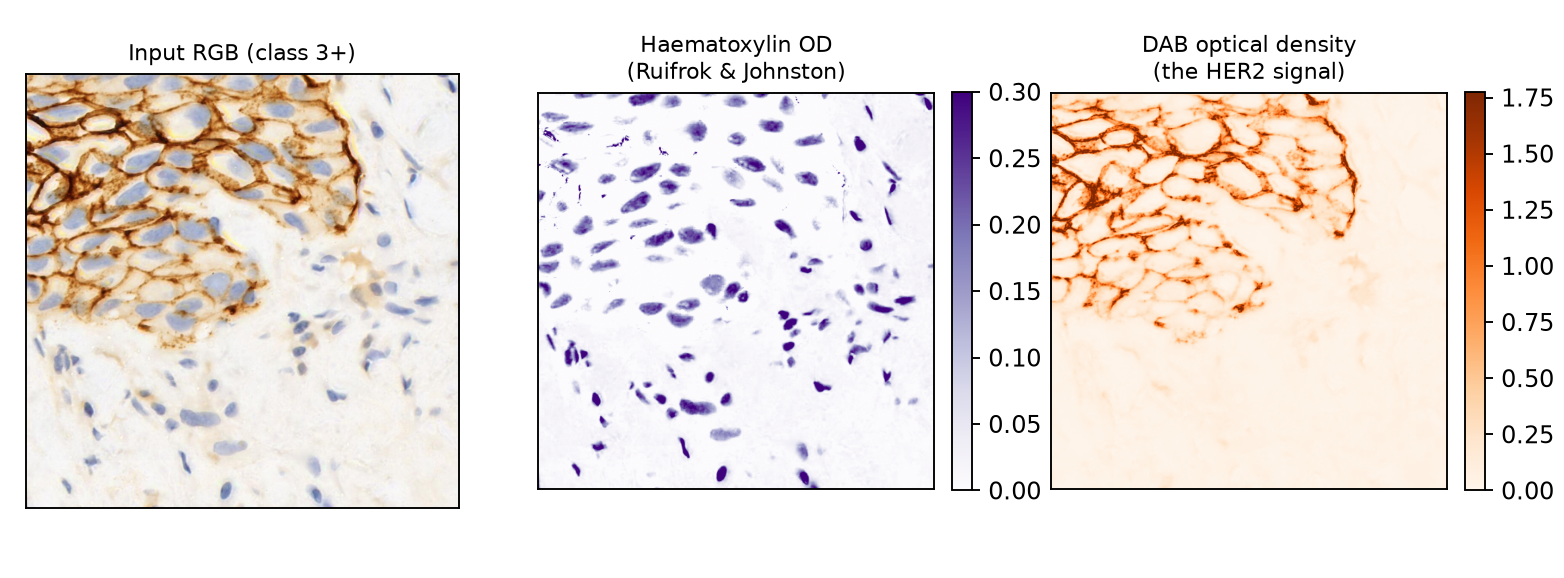
\includegraphics[width=\columnwidth]{../figures/stain_deconvolution.png}
\caption{Ruifrok--Johnston colour deconvolution on a real strongly-stained
(3+) patch: input RGB, recovered haematoxylin channel, and recovered DAB
channel.}
\label{fig:deconv}
\end{figure}

\subsection{Tissue Detection}

The tissue mask is the denominator of every percentage the system reports,
so its correctness matters more than its sophistication. An initial
implementation used Otsu thresholding \cite{otsu1979} on HSV saturation --
standard for low-magnification whole-slide thumbnails. It failed on
patch-level 40$\times$ IHC: the chosen threshold tracked staining intensity
rather than tissue presence, rising from $\approx$0.12 on faintly-stained
patches to $\approx$0.43 on strongly-stained ones, silently excluding
weakly-stained tissue from its own denominator. Fig.~\ref{fig:tissue}
demonstrates this on a real faintly-stained patch: the saturation-Otsu
mask covers only 34.9\% of the frame against 51.9\% for an
optical-density mask on the identical patch. We replaced saturation-Otsu
with detection by mean optical density across RGB, which responds to any
stain absorbing light rather than to which stain or how much.
Saturation-based detection remains available and is the correct choice at
low-magnification thumbnails, where the field is mostly glass; it is
simply the wrong tool at patch-level 40$\times$, where the field is
already almost all tissue.

\begin{figure}[t]
\centering
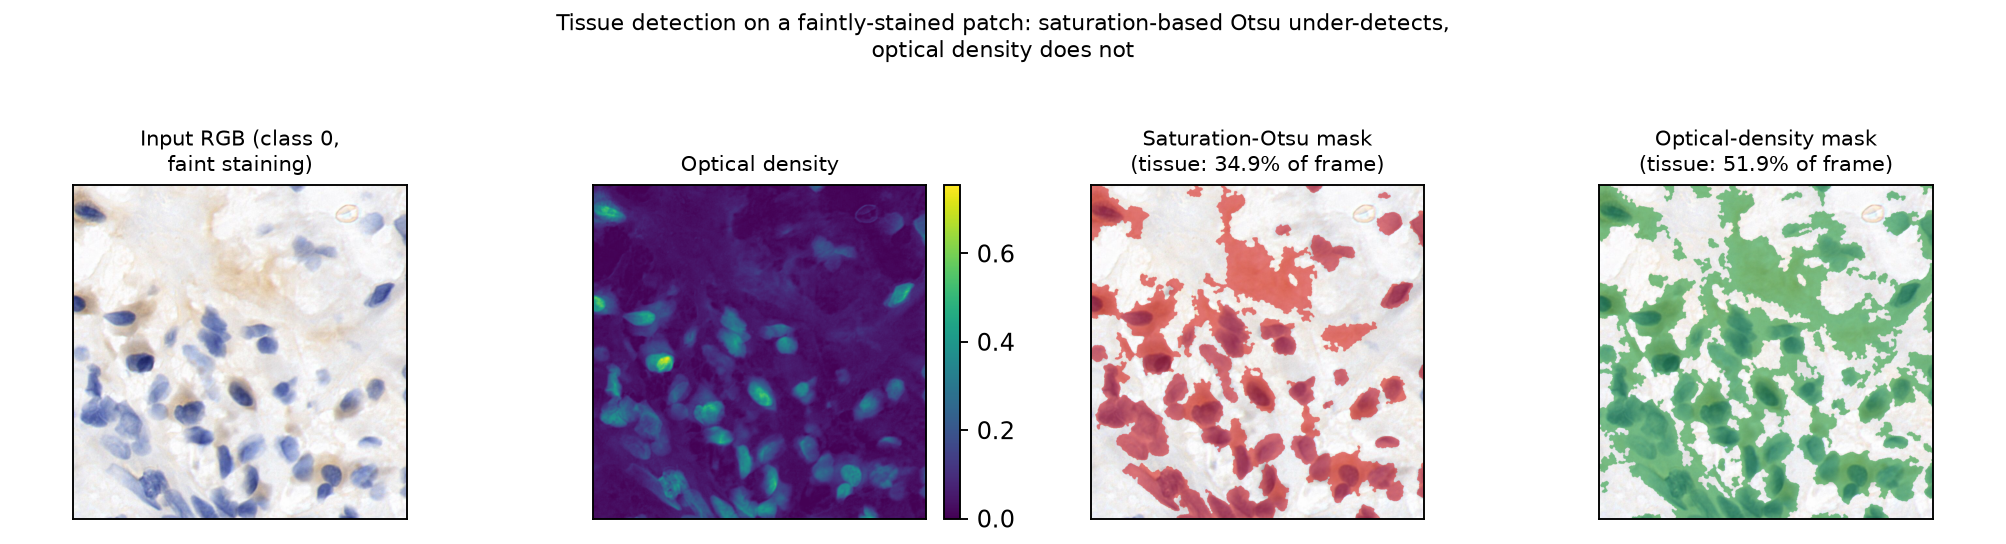
\includegraphics[width=\columnwidth]{../figures/tissue_detection_comparison.png}
\caption{Tissue detection on a real faintly-stained patch: saturation-Otsu
under-detects (34.9\%) relative to optical density (51.9\%) on the
identical frame.}
\label{fig:tissue}
\end{figure}

\subsection{The Classical Baseline}

A classical DAB-threshold classifier assigns each pixel one of five
intensity classes (background, negative, weak, moderate, strong) at fixed
optical-density cut points. This module plays three roles that matter to
keep distinct: it is the \textbf{pseudo-label generator} Phase 2 trains on;
it is the \textbf{experimental control} carried through every later
evaluation, since a learned model that merely agrees with the rule it was
trained on has demonstrated nothing; and it is the \textbf{area-percentage
engine} reused by the review-viewer and every report.

\subsection{Tiling}

Large images are split into fixed-size tiles by strided subsampling
(never averaging, which would blend stained and unstained pixels and shift
the optical densities the classes are defined on), tracking each tile's
position in both the working and original image frame -- bookkeeping a
future whole-slide stitching stage will depend on.

\section{Phase 2: Weakly-Supervised Segmentation}
\label{sec:phase2}

\subsection{No Pixel Annotations, No Slide Identifiers}

Two facts shape this phase entirely. First, there are no pixel-level
pathologist annotations anywhere in this project; the dense segmentation
targets are pseudo-labels -- literally the Phase 1 classical thresholder's
output, cached to disk so they can be inspected and disputed rather than
trusted blindly. A monotonic sanity check (mean stained area rising with
the dataset's own patch label, at two independently retiled
magnifications) is the only validation available in the absence of real
annotations. Second, HER2\_IHC\_40X carries no slide identifiers, so a true
slide-level train/validation split -- required so validation measures
generalization rather than memorisation of one slide's tissue -- is
impossible. The held-out set used throughout this paper is instead defined
by an inferred filename origin token (1{,}904 patches); the validation set
is a stratified random draw from the remainder and is explicitly labelled
\emph{not} leakage-free. Both caveats are written into every artifact a
training run produces.

\subsection{Model and Loss}

The segmentation model is a ResNet18 \cite{he2016} encoder with a U-Net
\cite{ronneberger2015} decoder, trained on cross-entropy, soft Dice, and
focal loss \cite{lin2017}, with dihedral-only augmentation (flips and
90\textdegree{} rotations, chosen because any colour or angle
transformation would shift the DAB optical densities the classes are
defined on). The loss composition is not incidental: Fig.~\ref{fig:balance}
shows the pixel-level class imbalance in the fit set (moderate (2+) is
3.6\% of pixels, against 80.8\% for background and negative combined),
which focal loss and, optionally, inverse-frequency weighting are
specifically intended to counteract. Section~\ref{sec:phase5} explains why
this architecture was adopted over an initial SegFormer baseline.
Fig.~\ref{fig:unetarch} diagrams the adopted encoder-decoder, including the
4-channel (RGB + DAB) input and exactly which stride the decoder stops at.

\begin{figure}[t]
\centering
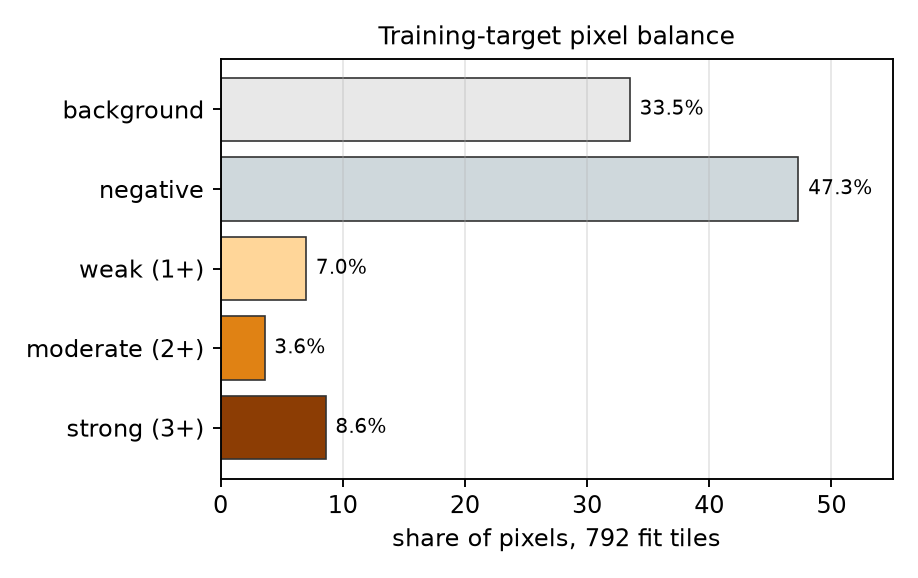
\includegraphics[width=\columnwidth]{../figures/pixel_class_balance.png}
\caption{Pixel-level class balance, 792 fit-set tiles. Moderate (2+) is
the rarest class by pixel count.}
\label{fig:balance}
\end{figure}

\begin{figure}[t]
\centering
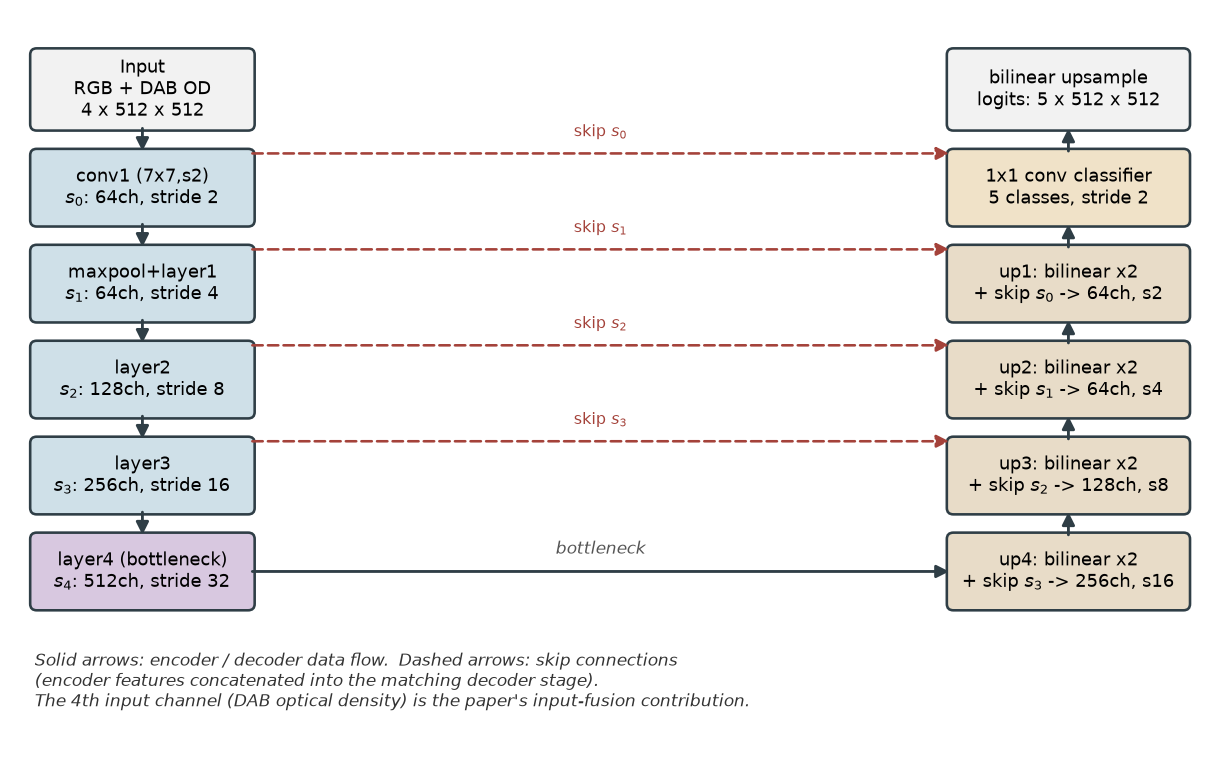
\includegraphics[width=\columnwidth]{../figures/unet_architecture.png}
\caption{ResNet18-UNet architecture, drawn from the model's actual forward
pass. The decoder stops at stride 2 (not stride 1), still twice
SegFormer's stride-4 output resolution, before a final non-learned
bilinear upsample of the logits.}
\label{fig:unetarch}
\end{figure}

\section{Phase 5: Architecture Comparison}
\label{sec:phase5}

An initial SegFormer-B0 \cite{xie2021} run diagnosed a specific failure:
its decode head predicts at $H/4\times W/4$ resolution before a single
bilinear upsample, and at the magnification first tried, thin HER2
membrane rims (1--3 pixels wide) were sub-pixel at that resolution before
ever reaching the loss. Retiling to native 40$\times$ resolution improved
the weak (1+) class substantially (IoU $0.030 \to 0.341$) but left moderate
(2+) essentially unlearned (IoU 0.0001, 253 of 21 million validation
pixels). A second architecture -- ResNet18 encoder, U-Net decoder, with
skip connections carrying full-resolution encoder features into the
decoder, plus the DAB optical-density channel fed as a fourth model input
alongside RGB -- was built and compared head-to-head against SegFormer,
same data, split, seed and epoch count.

\begin{table}[t]
\centering
\caption{Validation IoU, identical data/split/seed, 4 epochs, CPU-only.
Validation caveat: stratified random draw, not a held-out set (see
Section~\ref{sec:phase2}); used for architecture comparison, not as a
generalization estimate.}
\label{tab:archcompare}
\begin{tabular}{lrrr}
\toprule
Class & SegFormer-B0 & ResNet18-UNet & $\Delta$ \\
\midrule
Background & 0.852 & 0.861 & +0.009 \\
Negative & 0.815 & 0.839 & +0.024 \\
Weak (1+) & 0.341 & 0.666 & +0.325 \\
\textbf{Moderate (2+)} & \textbf{0.00006} & \textbf{0.589} & \textbf{+0.589} \\
Strong (3+) & 0.618 & 0.891 & +0.273 \\
\midrule
Tissue mean IoU & 0.443 & 0.746 & +0.303 \\
Pixel accuracy & 0.862 & 0.908 & +0.046 \\
\bottomrule
\end{tabular}
\end{table}

\begin{figure}[t]
\centering
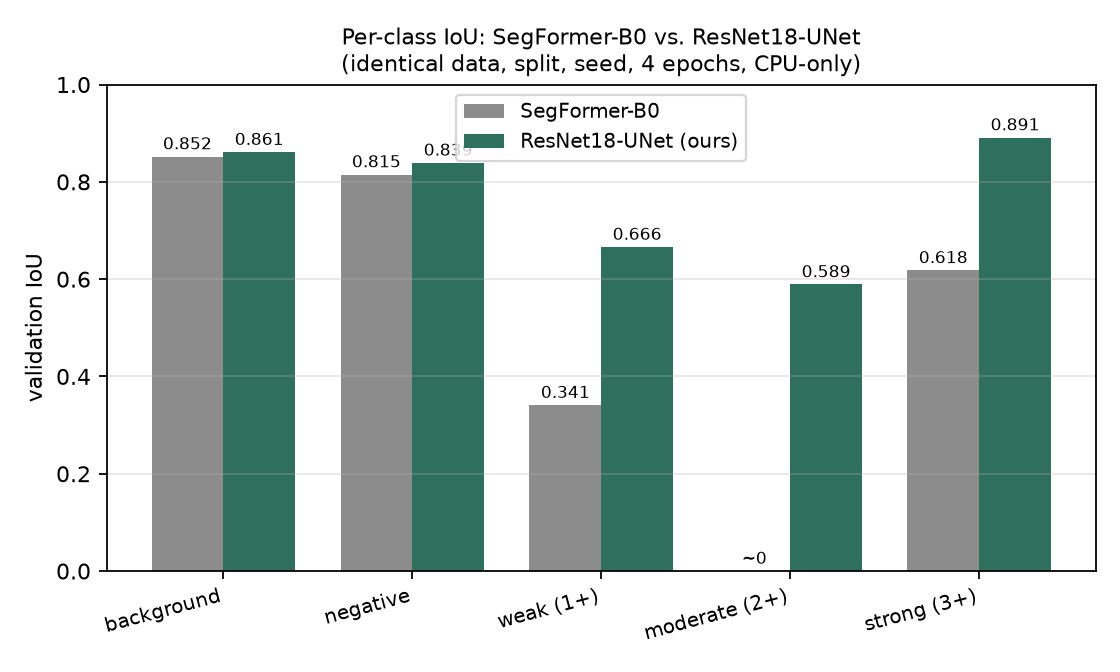
\includegraphics[width=\columnwidth]{../figures/architecture_comparison.png}
\caption{Per-class validation IoU, SegFormer-B0 vs. ResNet18-UNet.}
\label{fig:archcompare}
\end{figure}

U-Net won on every class (Table~\ref{tab:archcompare}, Fig.~\ref{fig:archcompare}),
most dramatically on moderate (2+) -- the class that decides reflex FISH
testing. \textbf{Decision: ResNet18-UNet was adopted as the sole
architecture; SegFormer was removed from the codebase entirely}, not kept
as a fallback. Beyond the accuracy gain, U-Net's plain
Conv2d/BatchNorm/ReLU construction exports to ONNX and quantizes with
fewer surprises than SegFormer's attention-based decoder, and removing it
dropped six now-unused dependencies. As Fig.~\ref{fig:efficiency}
quantifies, at $\approx$4.4\,s/image (forward + backward, CPU) against
SegFormer's $\approx$1.45\,s, U-Net costs $\approx3\times$ more per image
-- a real, stated price for the resolution it buys back, not an assumed
free upgrade.

\begin{figure}[t]
\centering
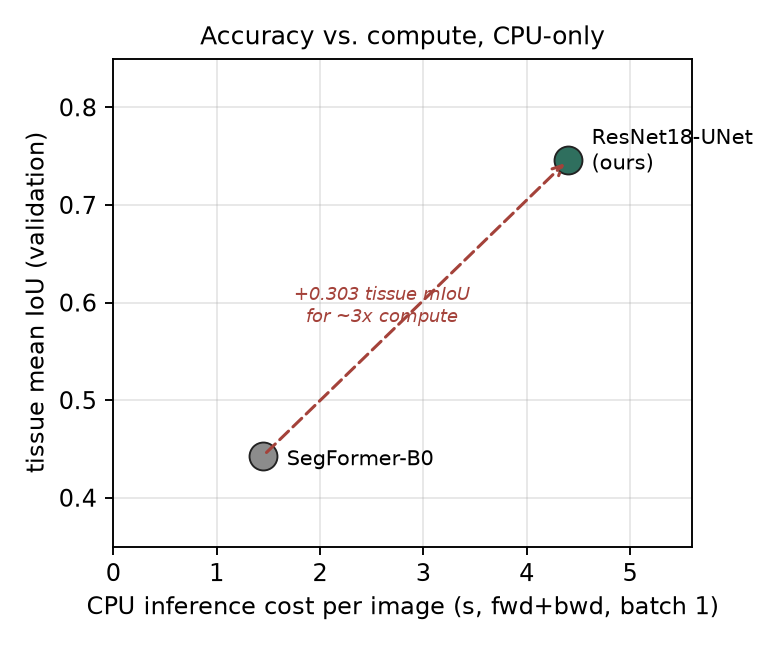
\includegraphics[width=0.92\columnwidth]{../figures/efficiency_accuracy.png}
\caption{Accuracy vs.\ CPU compute, both architectures. The adopted model
trades roughly $3\times$ compute for +0.303 tissue mean IoU.}
\label{fig:efficiency}
\end{figure}

Fig.~\ref{fig:training}--\ref{fig:preview} show training behaviour,
confusion structure, and qualitative predictions for the adopted model.
Losses fell monotonically on train and validation with no divergence.
Moderate (2+) remains the most-confused class (12.9\% of its pixels called
weak, 11.5\% called strong) but is now a genuine, non-degenerate row
in the confusion matrix rather than an empty one.

\begin{figure*}[t]
\centering
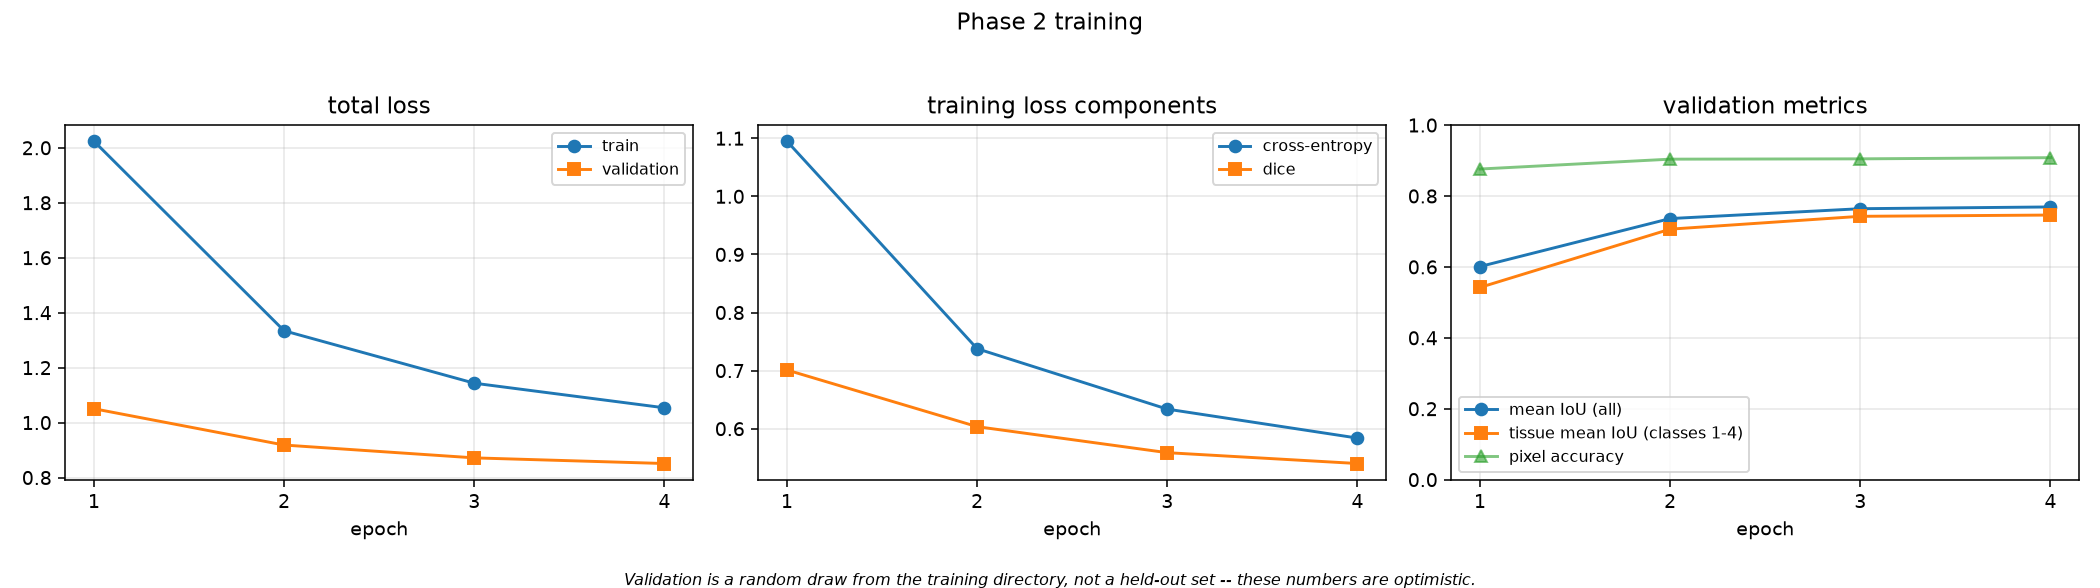
\includegraphics[width=0.95\textwidth]{../figures/unet_training_curves.png}
\caption{Training loss, loss components, and validation metrics, adopted
ResNet18-UNet model.}
\label{fig:training}
\end{figure*}

\begin{figure}[t]
\centering
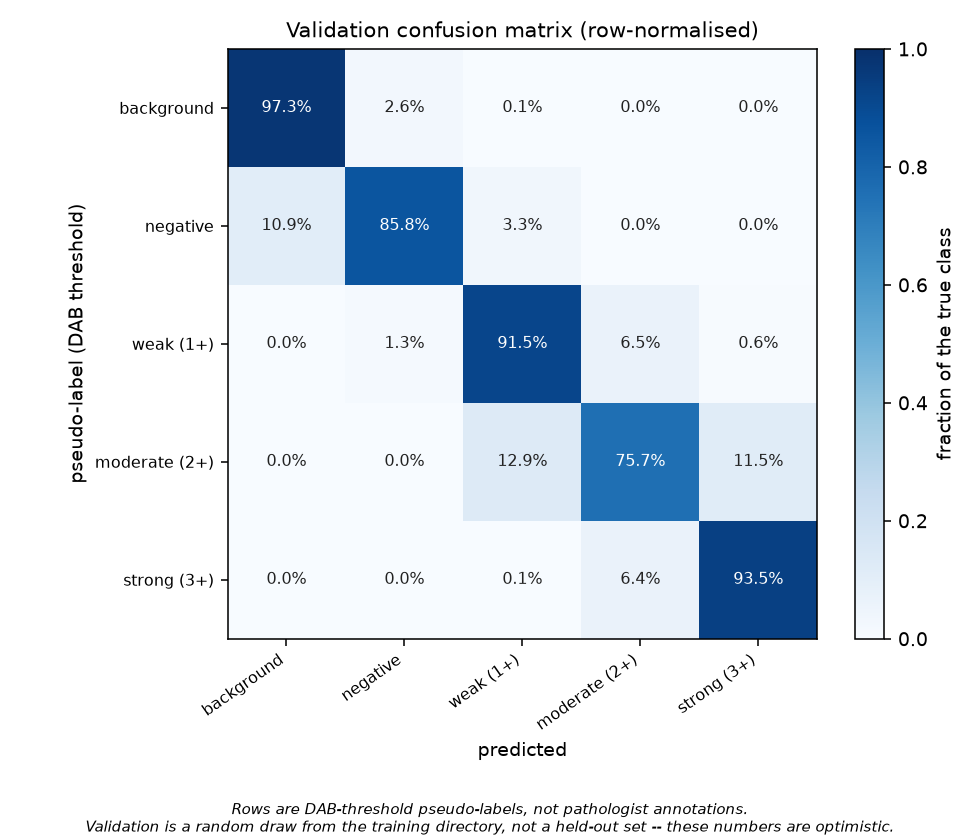
\includegraphics[width=\columnwidth]{../figures/unet_confusion.png}
\caption{Row-normalized validation confusion matrix, adopted model.}
\label{fig:confusion}
\end{figure}

\begin{figure*}[t]
\centering
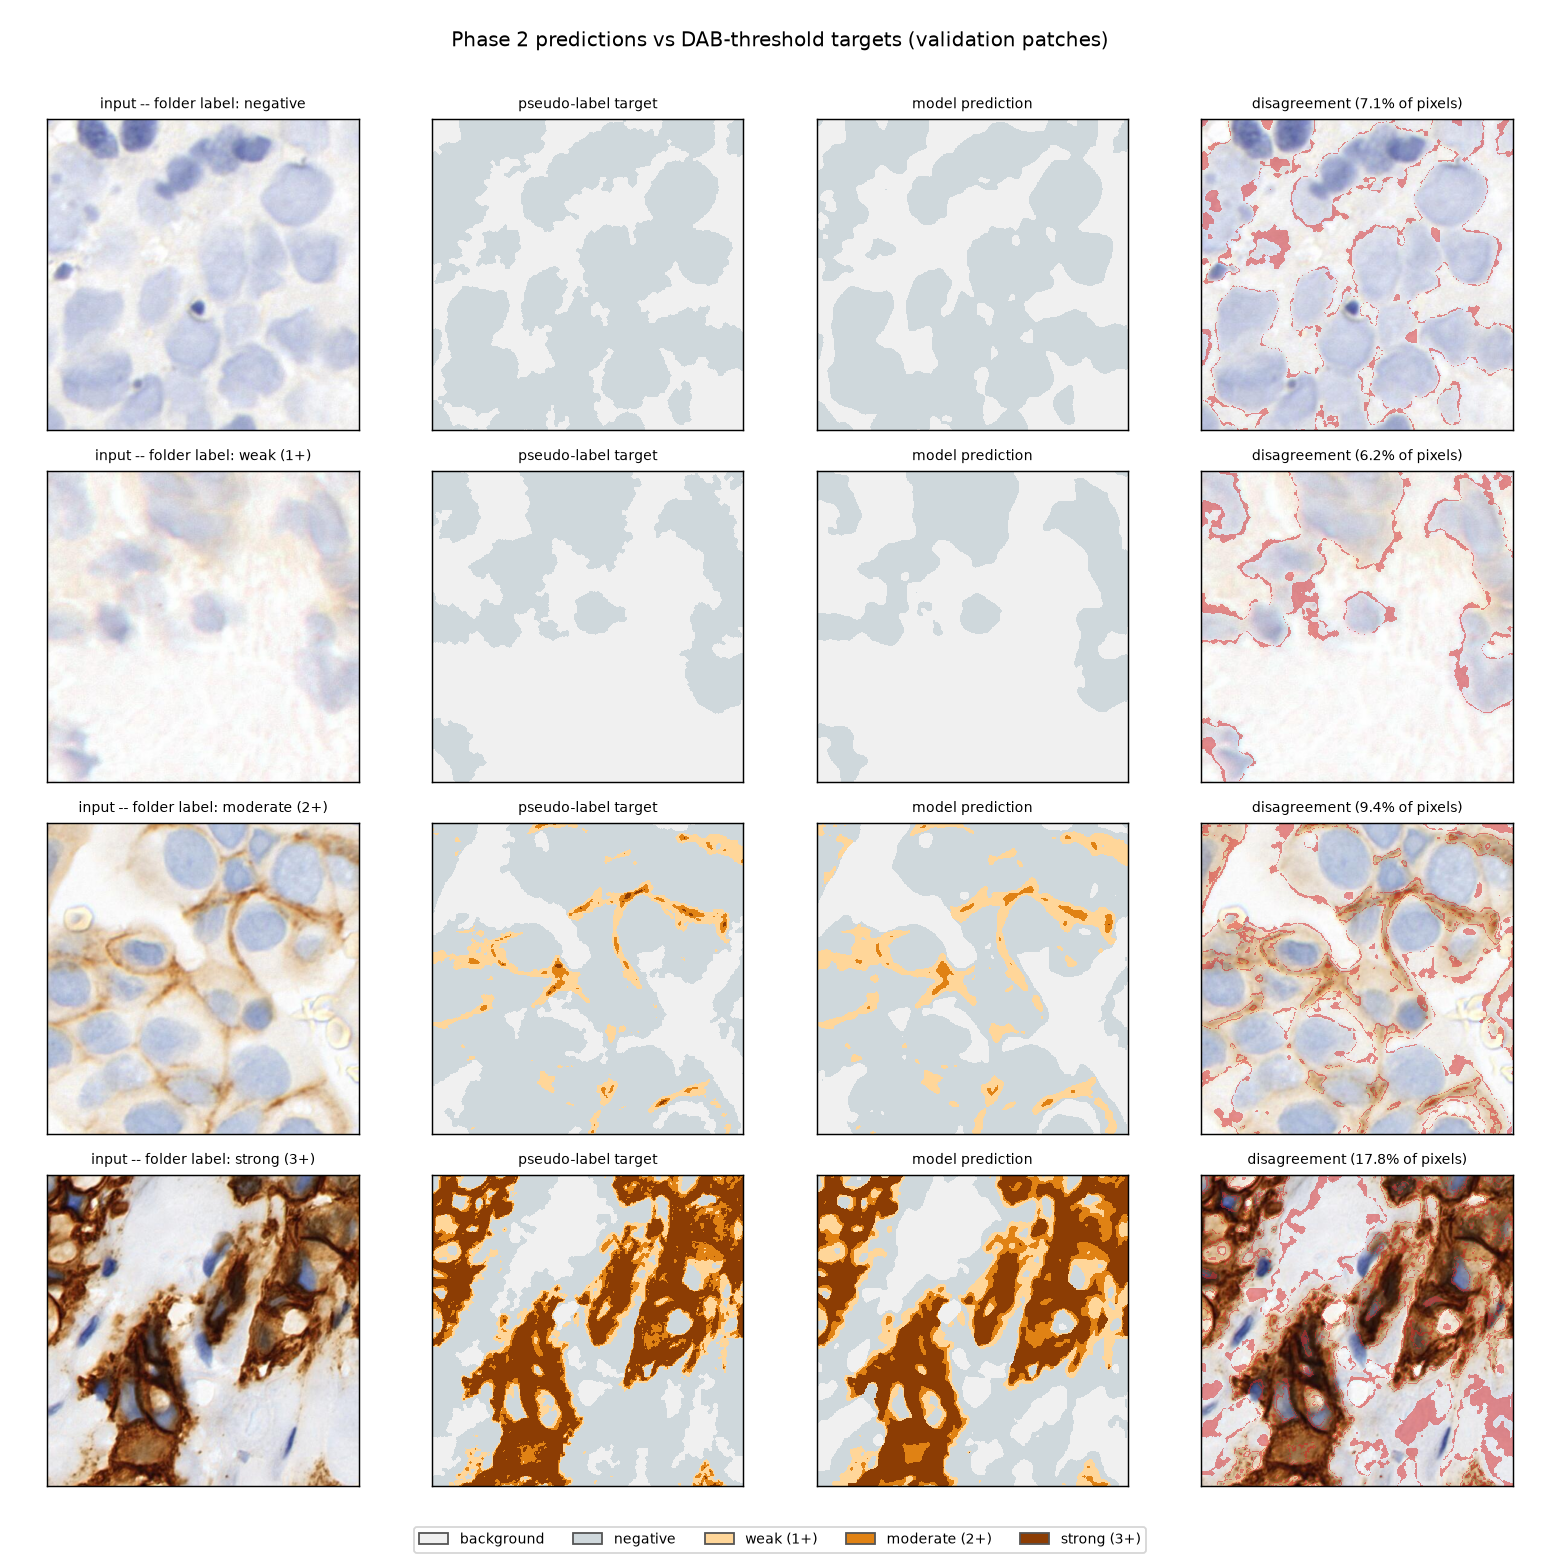
\includegraphics[width=0.95\textwidth]{../figures/unet_prediction_preview.png}
\caption{Input, pseudo-label target, prediction and disagreement, one
validation patch per intensity class, adopted model.}
\label{fig:preview}
\end{figure*}

\section{Phase 4: Evaluation Framework}
\label{sec:phase4}

\subsection{Stain Variation Across Provenance Groups}

HER2\_IHC\_40X carries no slide identifiers, so cross-slide stain variation
is measured across the dataset's 8 coarser provenance groups (label
$\times$ origin token) instead. A 6-dimensional stain descriptor (the
haematoxylin and DAB rows of a per-patch Macenko-estimated stain matrix
\cite{macenko2009}) is compared within- and between-group over 25 sampled
patches per group. The between-group mean descriptor distance (0.4230)
exceeds the within-group mean spread (0.2802), i.e.\ \texttt{variation\_exceeds\_noise}
is true (Fig.~\ref{fig:stainvar}). This result must be read carefully: the
8 groups are confounded with HER2 score by construction (a 3+ group is, by
definition, more heavily DAB-stained than a 0 group), so a stain
descriptor built from haematoxylin and DAB directions will partly detect
that confound rather than genuine cross-scanner or cross-institution
variation. The result is genuine evidence the descriptor is sensitive
enough to detect real variation of \emph{some} kind; only real
multi-institution data can say whether that kind is the cross-institution
shift the weighting in Section~\ref{sec:conformal} is meant to correct for.

\begin{figure}[t]
\centering
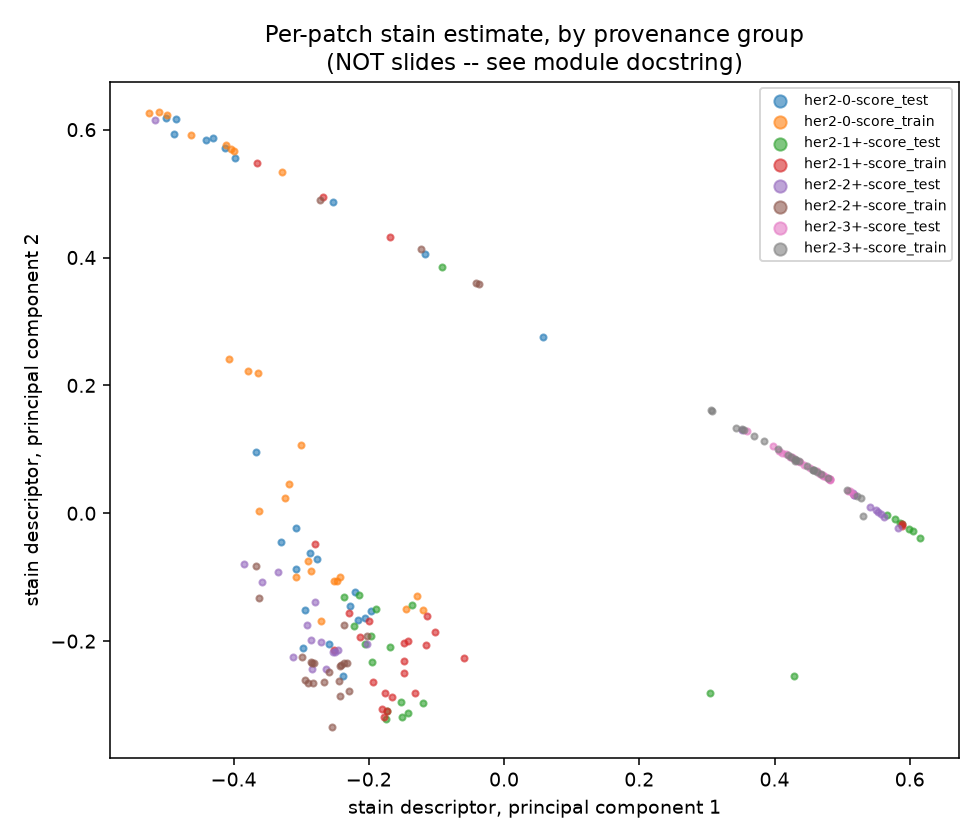
\includegraphics[width=\columnwidth]{../figures/stain_variation.png}
\caption{Between- vs.\ within-provenance-group stain descriptor distance,
HER2\_IHC\_40X.}
\label{fig:stainvar}
\end{figure}

\subsection{Stain-Shift-Weighted Conformal Prediction}
\label{sec:conformal}

We generalize binary, image-level inductive conformal prediction for HER2
status \cite{pintawong2025,vovk2005} to pixel-level, five-class
segmentation, using the hinge nonconformity score $s_c(x) = 1 - p_c(x)$
\cite{sadinle2019} and a per-class calibration quantile, and add
stain-shift-weighted calibration \cite{tibshirani2019}: each calibration
score is weighted by a Gaussian kernel over the stain descriptor distance
to the test patch, bandwidth set by the median pairwise calibration
distance. Calibration and evaluation spend the reserved holdout set once,
split into a calibration half and a test half that never touch the
fit/validation data. Because no pathologist pixel annotations exist,
calibration is against the same DAB-threshold pseudo-labels as training --
a prediction set achieving nominal coverage here is well-calibrated
against the rule the model was trained to imitate, not against clinical
truth. This is the same generalize-then-weight construction developed
independently in Section~IV of the companion methods paper on this
system's conformal predictor; we summarize the empirical result here and
refer the interested reader there for the full derivation.

\begin{table}[t]
\centering
\caption{Pixel-level conformal prediction, smoke-scale test set (52 tiles,
10{,}595{,}420 tissue pixels), evaluated against the adopted checkpoint.}
\label{tab:conformal}
\begin{tabular}{lrrrrrr}
\toprule
& \multicolumn{3}{c}{Unweighted} & \multicolumn{3}{c}{Weighted} \\
$\alpha$ & Misc. & Amb. & Acc. & Misc. & Amb. & Acc. \\
\midrule
0.05 & 0.044 & 0.110 & 0.971 & 0.047 & 0.106 & 0.969 \\
0.10 & 0.089 & 0.072 & 0.950 & 0.093 & 0.072 & 0.949 \\
0.20 & 0.183 & 0.142 & 0.953 & 0.189 & 0.151 & 0.955 \\
0.50 & 0.489 & 0.480 & 0.983 & 0.491 & 0.482 & 0.983 \\
\bottomrule
\end{tabular}
\end{table}

Table~\ref{tab:conformal} shows miscoverage tracking $\alpha$ closely
(e.g.\ 0.044 at $\alpha=0.05$) -- the finite-sample coverage guarantee
holding on real held-out data -- and weighted vs.\ unweighted staying
close at every row, which is the expected, honest result of running a
cross-institution correction on HER2\_IHC\_40X's single-source data: there
is no genuine shift here for the weighting to correct. The mechanism is
validated separately on deliberately-constructed synthetic multi-source
data in our test suite. This evaluation is smoke-scale (52 of
$\approx$1{,}900 available held-out test tiles); a full-scale run is
software-ready but unrun, a multi-hour CPU job at this per-tile cost.

\subsection{Offline ASCO/CAP Mapping and Expert Agreement}

The model's per-class area percentages are mapped to an ASCO/CAP 2018
\cite{wolff2018} category by area-percentage thresholds analogous to the
guideline's tumour-cell-percentage rule: 3+ if strong-staining area exceeds
10\%; else 2+ if moderate-or-above area is at least 10\%; else 1+ if
weak-or-above area exceeds 10\%; else 0. \textbf{This mapping is
deliberately never imported into the review-viewer application}
(Section~\ref{sec:app}) -- exposing a \texttt{cap\_score} field in the live
API would be the system's one enforced rule, broken under a different
field name; formally, it would implement the very $h$ that
Section~\ref{sec:principle} forbids inside $g_\theta$. It exists only as
an offline script a person runs and reads. Agreement with expert ground
truth is computed as exact agreement, within-one-category agreement, and
quadratic-weighted Cohen's kappa \cite{cohen1968} against
\texttt{reviews.jsonl}, the file the review-viewer's
\texttt{/api/review} endpoint appends a record to every time a pathologist
confirms a score. As of writing, that file has zero real entries, because
no pathologist has yet used the viewer -- the pipeline is complete and
tested against synthetic review data, and activates automatically the day
a real review is recorded. We state this plainly rather than substituting
a synthetic number for a clinical one. A further, permanent caveat:
ASCO/CAP scoring is defined on percentage of \emph{tumour cells}; every
measurement in this system is percentage of \emph{tissue area}, which
includes stroma, and the two diverge whenever stroma content varies --
which it does substantially here (mean tissue fraction 0.45 in class 0 to
0.79 in class 3+).

\section{The Review-Viewer Application}
\label{sec:app}

\subsection{Design}

The review-viewer is a local, dependency-free web application
(\texttt{http.server.ThreadingHTTPServer}; no framework, no CDN, nothing
fetched from the internet at runtime), because the machines this system is
meant to be demonstrated on -- hospital and college computers -- are
exactly where an internet dependency or a heavyweight framework is a
failure mode. It binds to \texttt{127.0.0.1} by default and warns loudly if
pointed elsewhere: displaying medical images and recording clinical
opinions with no authentication and no transport security makes this a
local demonstration and review aid, not a deployable clinical service, by
design.

\subsection{Workflow}

Fig.~\ref{fig:appflow} traces one review end to end, from opening the
viewer to an optional PDF export. A pathologist opens the viewer, selects a
sample patch or uploads an image,
and receives four panels -- original, detected tissue, model intensity map,
classical baseline -- and one area-percentage table, \textbf{model and
baseline always shown side by side, never one without the other}: because
the model trains on the baseline's own output, agreement between the two
is agreement with the rule the model imitates, not evidence of clinical
accuracy, and hiding that comparison behind an optional toggle would let a
viewer see only the flattering number. The moderate (2+) row is flagged
inline in the table itself (an amber warning), not only in a footnote,
because a caveat at the page bottom is a caveat a screenshot crops out. The
pathologist then completes an explicit review form -- a reviewer identity
plus a chosen score, with "cannot assess from this field" offered as a
first-class option -- and only that submission writes a record to
\texttt{reviews.jsonl}. A PDF export renders the identical payload the live
API returns, carrying the same never-a-score guarantee, verified directly
in the test suite.

\begin{figure}[t]
\centering
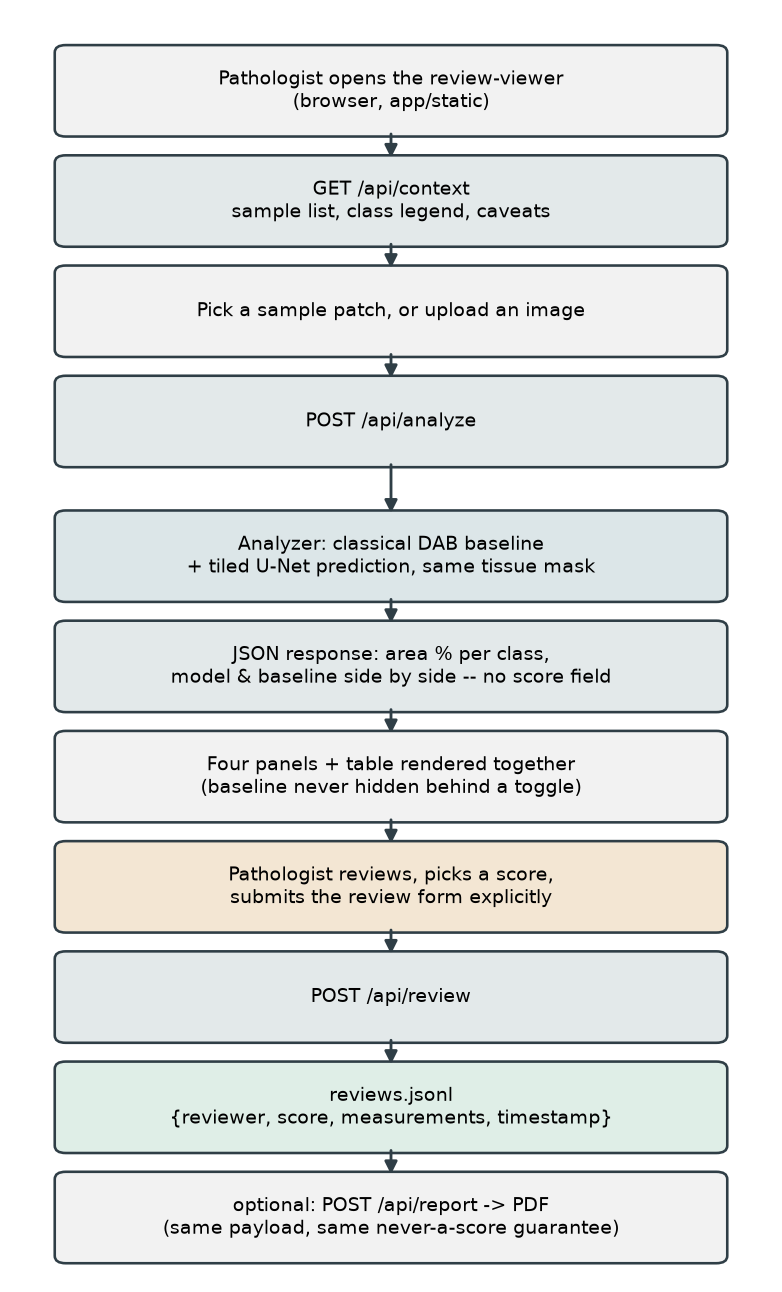
\includegraphics[width=0.72\columnwidth]{../figures/app_flow.png}
\caption{Review-viewer request flow, one review end to end. A HER2 score
enters the system only at the explicit-submit step; nothing upstream of
it can create one.}
\label{fig:appflow}
\end{figure}

\subsection{The One Rule, Enforced as Code}

The system's central design constraint -- assistive, never autonomous, and
formally $h \notin \text{range reachable from } g_\theta$
(Section~\ref{sec:principle}) -- is checked, not just stated: the live
JSON API is scanned on every test run for the literal keys
\texttt{score}, \texttt{her2\_score}, \texttt{verdict}, and
\texttt{diagnosis}, and the build fails if any appear anywhere in the
response. The review UI's submit action is likewise tested to require an
explicit form submission with a reviewer identity; no code path can
record a review automatically. We treat these as load-bearing
specification, in the same category as ordinary correctness tests (tiled
predictions cover the whole image; splits contain no leaked patches;
weights resolve to the expected length), because they are exactly the
properties a well-intentioned future UI or API change could erode without
anyone noticing until a pathologist is looking at a silently overconfident
screen.

\subsection{Packaging}

The application is containerized (\texttt{Dockerfile} plus
\texttt{docker-compose.yml}), publishing on \texttt{127.0.0.1} on the host
only, matching the server's own no-broader-exposure stance. PyTorch is
installed explicitly from the CPU wheel index rather than plain PyPI, since
a naive \texttt{pip install -r requirements.txt}-only image would silently
lack it. Docker packaging is written and unit-verified but has not been
run to completion end to end on real hardware, as no Docker installation
was available on the original development machine; we report this as an
open item rather than a completed one.

\section{System-Level Results}

\begin{table}[t]
\centering
\caption{Coverage against the project's original nine-item brief.}
\label{tab:coverage}
\small
\begin{tabular}{p{0.62\columnwidth}l}
\toprule
Scope item & Status \\
\midrule
Digitize IHC slides into WSI & Blocked on data \\
Tissue detection & Done \\
Stain normalization + deconvolution & Done \\
Patch extraction, patch-level analysis & Done \\
Intensity classification (weak/mod./strong) & Done, 1 class weak \\
Tissue area \% per intensity category & Done \\
Heatmaps + slide-level summary & Partial \\
Validation vs.\ pathologist annotation & Built, 0 real data \\
Integration as pre-scoring workflow tool & Done \\
\bottomrule
\end{tabular}
\end{table}

Table~\ref{tab:coverage} summarizes the honest state of every item in the
project's original brief: 6 of 9 are done, 1 (slide-level heatmaps) is
genuinely partial pending whole-slide stitching, and 2 (real-slide
digitization; validation against real pathologist annotation) are blocked
on data no engineering effort in this system can substitute for -- they
are ready to activate the moment that data exists, not unstarted. The
system's test suite -- 283 tests at time of writing, spanning every phase
above -- is treated as the project's actual specification: a real category
of these tests encodes the framing constraints of
Section~\ref{sec:app} as literal assertions, not only ordinary
correctness checks, specifically so a future change cannot silently erode
them.

\section{Discussion: Honesty as an Engineering Principle}

Two properties of this system are, we argue, as important as any single
accuracy number. First, \textbf{every reported number carries the
conditions it was measured under}, written into the artifact itself, not
only into this paper: validation metrics are marked not-leakage-free at
the point they are computed; conformal coverage results carry a
pseudo-label calibration caveat; CAP-mapped agreement carries a
tissue-area-not-tumour-cell-area caveat. A number copied out of this
system's output directory arrives with its caveat attached, because the
caveat is written into the same file as the number. Second, \textbf{framing
constraints are tested, not merely documented} (Section~\ref{sec:app}): the
distinction between "this tool measures" and "this tool scores" is the
entire clinical safety argument for building it this way, and encoding
that distinction as an executable test is what keeps a future,
well-intentioned change from crossing it by accident.

\section{Threats to Validity}
\label{sec:threats}

We organize the system's limitations by the standard
construct/internal/external/statistical validity taxonomy, since it makes
explicit which threats are resolvable by more engineering and which are
not.

\textbf{Construct validity.} Every accuracy, coverage, and agreement number
this system reports is a measurement of agreement with a classical
DAB-threshold rule (Section~\ref{sec:phase2}) or, in the case of CAP
agreement, with the dataset's own folder label -- not with independent
pathologist ground truth, which does not yet exist for this project in
pixel or, for CAP agreement, case form. Similarly, ASCO/CAP percentages
are defined on tumour-cell area; this system reports tissue area, and the
two diverge whenever stroma content varies.

\textbf{Internal validity.} The held-out set is inferred from filename
structure on a dataset with no slide identifiers, not a verified
slide-level partition -- validation and holdout performance may in part
reflect generalization across patches of the same slide rather than
across slides.

\textbf{External validity.} Every result in this paper is validated
against HER2\_IHC\_40X, a public single-source substitute, not the
reference site's 84 (still undigitized) slides; the stain-shift-weighted
conformal predictor has no genuine cross-institution shift on this dataset
to demonstrate a benefit against and is validated on synthetic shift only;
and Docker packaging is written and unit-verified but not run to
completion end to end on real hardware.

\textbf{Statistical conclusion validity.} The conformal evaluation is
real, computed against the actual deployed checkpoint, but over 52 of
$\approx$1{,}900 available held-out test tiles -- a full-scale run is
software-ready but unrun, a multi-hour CPU job at this per-tile cost. No
result in this paper is averaged over multiple seeds, owing to the
CPU-only compute budget.

\textbf{Blocked on data, not on engineering.} Two items in
Table~\ref{tab:coverage} -- real whole-slide-image data and real
pathologist reviews (\texttt{reviews.jsonl} has zero real entries) -- are
threats no further engineering in this system can resolve; both pipelines
are complete and tested and activate automatically the moment the
corresponding data exists.

\textbf{The remaining open question.} Moderate (2+) remains the weakest
stained class (IoU 0.589 against 0.67--0.89 for the others) and is exactly
the category that decides reflex FISH testing; it is resolved as
\emph{learnable}, not as solved.

\section{Broader Impact and Ethical Considerations}

The system's central engineering decision -- that $g_\theta$
(Section~\ref{sec:principle}) never implements $h$ -- is also its central
ethical safeguard: the risk we designed most deliberately against is
automation bias, where a sufficiently accurate-looking assistive output is
treated as a diagnosis by a time-pressured reviewer. Making the "measures,
does not score" boundary a tested property of the API, not only of the
interface copy, is intended to make that boundary durable across future
changes made by people who were not in the room for this design decision.
Conformal prediction reinforces the same goal at the statistical level: a
wide prediction set at a clinically relevant significance level is a
legitimate, intended output -- the system declining to be confident -- not
a failure to be tuned away.

Beyond automation bias, two considerations bear on responsible deployment.
\textbf{Representativeness:} HER2\_IHC\_40X's demographic and
institutional provenance is not documented at the level clinical
deployment would require, and no result in this paper should be read as
evidence of population-level clinical validity. \textbf{Equity of
access:} every component in this pipeline runs on CPU-only commodity
hardware by design (Section~\ref{sec:phase5}), which we view as directly
relevant to whether AI-assisted pathology tooling remains reachable for
resource-constrained departments rather than only for institutions with
GPU infrastructure. Finally, the review-viewer's explicit no-authentication,
no-transport-security, localhost-only design (Section~\ref{sec:app}) is a
deliberate scope limitation, not an oversight: it is a demonstration and
review aid for a controlled setting, and any path toward broader clinical
deployment would require an authentication, auditing, and data-governance
layer this paper does not claim to provide.

\section{Conclusion and Future Work}

BioMarkHER2 demonstrates that a defensible, pathologist-in-the-loop HER2
IHC pre-scoring system can be built end to end -- preprocessing, weakly
supervised segmentation, calibrated uncertainty, offline clinical-guideline
mapping, and a tested, demonstrable application -- entirely under weak
supervision and CPU-only compute, with every result reported alongside the
conditions it was measured under and the validity threats organized
systematically rather than left implicit. Immediate future work is:
whole-slide tiling and stitching against synthetic mosaics, buildable now
without waiting for real WSIs; a full-scale conformal evaluation over the
entire reserved holdout set; multi-seed replication of the architecture
comparison; a per-cell membrane-completeness reformulation of the
moderate (2+) class, closer to how ASCO/CAP itself defines the score; and,
as real data arrives, replacing pseudo-label calibration with pathologist
pixel annotation and exercising the stain-shift-weighted conformal
predictor on genuine multi-institution variation.

\section*{Acknowledgment}
Acknowledgments withheld pending submission.

\begin{thebibliography}{00}

\bibitem{wolff2018} A. C. Wolff \emph{et al.}, ``Human Epidermal Growth
Factor Receptor 2 Testing in Breast Cancer: ASCO/CAP Clinical Practice
Guideline Focused Update,'' \emph{J. Clin. Oncol.}, vol. 36, no. 20,
pp. 2105--2122, 2018.

\bibitem{bera2019} K. Bera, K. A. Schalper, D. L. Rimm, V. Velcheti, and
A. Madabhushi, ``Artificial intelligence in digital pathology -- new tools
for diagnosis and precision oncology,'' \emph{Nat. Rev. Clin. Oncol.},
vol. 16, pp. 703--715, 2019.

\bibitem{selcuk2024} S. Yoruc Selcuk \emph{et al.}, ``Automated HER2
Scoring in Breast Cancer Images Using Deep Learning and Pyramid Sampling,''
\emph{BME Front.}, 2024.

\bibitem{mridha2022} M. F. Mridha, M. K. Morol, M. A. Ali, and M. S. H.
Shovon, ``convoHER2: A Deep Neural Network for Multi-Stage Classification
of HER2 Breast Cancer,'' arXiv:2211.10690, 2022.

\bibitem{han2021} C. Han \emph{et al.}, ``Multi-Layer Pseudo-Supervision
for Histopathology Tissue Semantic Segmentation using Patch-level
Classification Labels,'' arXiv:2110.08048, 2021.

\bibitem{hetz2024} M. J. Hetz, T. C. Bucher, and T. J. Brinker,
``Multi-domain stain normalization for digital pathology: A
cycle-consistent adversarial network for whole slide images,'' \emph{Med.
Image Anal.}, vol. 94, p. 103149, 2024.

\bibitem{mossina2025} L. Mossina and C. Friedrich, ``Conformal Prediction
for Image Segmentation Using Morphological Prediction Sets,'' in
\emph{Proc. MICCAI}, 2025.

\bibitem{borden2026} B. J. Borden, J. B. Graham-Knight, P. Lasserre,
S. Lucas, and R. D. Rajapakshe, ``Uncertainty quantification of U-Net based
segmentation tool using conformal prediction,'' \emph{J. Appl. Clin. Med.
Phys.}, vol. 27, no. 7, p. e70663, 2026.

\bibitem{pintawong2025} P. Pintawong \emph{et al.}, ``Conformal Prediction
for Uncertainty Quantification and Reliable HER2 Status Classification in
Breast Cancer IHC Images,'' \emph{IEEE Access}, 2025.

\bibitem{ruifrok2001} A. C. Ruifrok and D. A. Johnston, ``Quantification of
histochemical staining by color deconvolution,'' \emph{Anal. Quant. Cytol.
Histol.}, vol. 23, no. 4, pp. 291--299, 2001.

\bibitem{macenko2009} M. Macenko \emph{et al.}, ``A method for normalizing
histology slides for quantitative analysis,'' in \emph{Proc. IEEE Int.
Symp. Biomedical Imaging (ISBI)}, 2009, pp. 1107--1110.

\bibitem{reinhard2001} E. Reinhard, M. Adhikhmin, B. Gooch, and P. Shirley,
``Color transfer between images,'' \emph{IEEE Comput. Graph. Appl.},
vol. 21, no. 5, pp. 34--41, 2001.

\bibitem{otsu1979} N. Otsu, ``A threshold selection method from gray-level
histograms,'' \emph{IEEE Trans. Syst., Man, Cybern.}, vol. 9, no. 1,
pp. 62--66, 1979.

\bibitem{ronneberger2015} O. Ronneberger, P. Fischer, and T. Brox, ``U-Net:
Convolutional networks for biomedical image segmentation,'' in \emph{Proc.
MICCAI}, 2015, pp. 234--241.

\bibitem{he2016} K. He, X. Zhang, S. Ren, and J. Sun, ``Deep residual
learning for image recognition,'' in \emph{Proc. IEEE CVPR}, 2016,
pp. 770--778.

\bibitem{xie2021} E. Xie, W. Wang, Z. Yu, A. Anandkumar, J. M. Alvarez, and
P. Luo, ``SegFormer: Simple and efficient design for semantic segmentation
with transformers,'' in \emph{Proc. NeurIPS}, 2021.

\bibitem{lin2017} T.-Y. Lin, P. Goyal, R. Girshick, K. He, and P. Doll\'ar,
``Focal loss for dense object detection,'' in \emph{Proc. IEEE ICCV}, 2017,
pp. 2980--2988.

\bibitem{vovk2005} V. Vovk, A. Gammerman, and G. Shafer, \emph{Algorithmic
Learning in a Random World}. New York, NY, USA: Springer, 2005.

\bibitem{sadinle2019} M. Sadinle, J. Lei, and L. Wasserman, ``Least
ambiguous set-valued classifiers with bounded error levels,'' \emph{J. Am.
Stat. Assoc.}, vol. 114, no. 525, pp. 223--234, 2019.

\bibitem{tibshirani2019} R. J. Tibshirani, R. Foygel Barber, E. Cand\`es,
and A. Ramdas, ``Conformal prediction under covariate shift,'' in
\emph{Proc. NeurIPS}, 2019.

\bibitem{cohen1968} J. Cohen, ``Weighted kappa: Nominal scale agreement
with provision for scaled disagreement or partial credit,'' \emph{Psychol.
Bull.}, vol. 70, no. 4, pp. 213--220, 1968.

\end{thebibliography}

\end{document}
